\documentclass[11pt,twocolumn]{article}

\usepackage[letterpaper,margin=0.72in,top=0.74in,bottom=0.78in,columnsep=0.25in]{geometry}
\usepackage[T1]{fontenc}
\usepackage{newtxtext,newtxmath}
\usepackage{microtype}
\usepackage{amsmath,mathtools}
\usepackage{booktabs}
\usepackage{graphicx}
\usepackage{subcaption}
\usepackage{tabularx}
\usepackage{enumitem}
\usepackage{xcolor}
\usepackage{xurl}
\usepackage{hyperref}
\usepackage{fancyhdr}
\usepackage{titlesec}
\usepackage[round,authoryear]{natbib}

\definecolor{linkblue}{RGB}{32,84,147}
\hypersetup{colorlinks=true,linkcolor=linkblue,urlcolor=linkblue,citecolor=linkblue}
\graphicspath{{figures/}}
\captionsetup{font=small,labelfont=bf,justification=justified,singlelinecheck=false}
\captionsetup[subfigure]{font=small,labelfont=bf}
\setlength{\textfloatsep}{8pt plus 2pt minus 2pt}
\setlength{\floatsep}{7pt plus 2pt minus 2pt}
\setlength{\intextsep}{7pt plus 2pt minus 2pt}
\setlength{\abovecaptionskip}{4pt}
\setlength{\belowcaptionskip}{0pt}
\setlist{leftmargin=*,nosep}
\titleformat{\section}{\large\bfseries}{\thesection}{0.45em}{}
\titleformat{\subsection}{\normalsize\bfseries}{\thesubsection}{0.45em}{}
\titlespacing*{\section}{0pt}{8pt plus 2pt minus 2pt}{3pt}
\titlespacing*{\subsection}{0pt}{6pt plus 2pt minus 2pt}{2pt}
\pagestyle{fancy}
\fancyhf{}
\fancyhead[L]{\small Repairing Activation Steering}
\fancyhead[R]{\small leolazz}
\fancyfoot[C]{\thepage}
\renewcommand{\headrulewidth}{0.3pt}
\setlength{\headheight}{13pt}
\linespread{1.025}

\newcommand{\dNLL}{\Delta\mathrm{NLL}}
\newcommand{\KL}{D_{\mathrm{KL}}}
\newcommand{\method}[1]{\textsc{#1}}

\title{\vspace{-1.2em}\textbf{Repairing Activation Steering with\\Downstream-Aware Denoising}\vspace{-0.4em}}
\author{leolazz\\T-Lab Mechanistic Interpretability Research Project}
\date{}

\begin{document}
\maketitle
\thispagestyle{fancy}

\begin{abstract}
Activation steering modifies language-model behavior by adding a direction to an intermediate representation, but sufficiently strong interventions can substantially distort downstream computation. We ask whether this collateral damage can be repaired without erasing the intended intervention. Using GPT-2 Small and sparse-autoencoder (SAE) directions at \texttt{blocks.6.hook\_resid\_pre}, we compare raw steering, reconstruction denoisers, intervention-conditioned denoisers, downstream distribution matching, and explicit feature-retention constraints. Relative raw steering produces mean $\dNLL=7.01$. A direction- and strength-conditioned reconstruction model remains at $6.91$, whereas replacing reconstruction with downstream KL reduces mean $\dNLL$ to $2.07$. Adding soft retention leaves degradation essentially unchanged at $2.06$ while increasing mean target-feature retention from $1.011$ to $1.115$. On a designated 20-direction, 3,200-example unseen holdout, the selected method recovers $4.32$ mean $\dNLL$ relative to raw steering (95\% CI $[2.93,5.79]$), improves all 20 directions, and increases mechanistic retention by $0.108$ (95\% CI $[0.077,0.139]$). A separate sentiment direction reproduces the central KL-over-reconstruction result. The evidence supports a functional formulation of repair: \emph{functional steering repair is not the same problem as activation reconstruction}.
\end{abstract}

\section{Introduction}
Activation steering controls language-model behavior without updating the underlying model parameters \citep{turner2023activation,rimsky2024caa}. Given an intermediate representation $h$ and direction $v$, a standard intervention is
\begin{equation}
  h_{\mathrm{steered}} = h + \alpha v.
\end{equation}
Increasing intervention magnitude may strengthen the desired effect, but also perturbs the representation consumed by every subsequent transformer layer. Strong steering can therefore alter next-token probabilities, negative log-likelihood, activation geometry, and free-running generation, reflecting a broader effectiveness--fluency tradeoff in language-model conditioning \citep{macocco2026tradeoff}.

The central question is whether one can repair the unintended downstream consequences while retaining the component responsible for the intended intervention. A direct reconstruction model,
\begin{equation}
  D(h_{\mathrm{steered}}) \approx h,
\end{equation}
is ambiguous: moving back toward $h$ may reduce damage by removing the intervention itself. Moreover, Euclidean proximity in activation space need not imply functional similarity after the nonlinear downstream transformer.

We instead provide intervention metadata to the denoiser and optimize the distribution produced downstream of the repaired state. Controlled ablations show that conditioning alone is insufficient. The dominant improvement comes from a downstream KL objective; a separate retention constraint then limits how much intended signal the repair may erase.

Our contributions are:
\begin{enumerate}
  \item an intervention-aware formulation $D(x,v,s)$ for steering repair;
  \item a causal ablation separating conditioning, reconstruction, downstream KL, and retention;
  \item a frozen 20-direction unseen SAE holdout with paired uncertainty;
  \item a narrow cross-concept confirmation on one independent sentiment direction; and
  \item an external semantic proxy showing that SAE feature retention is not semantic ground truth.
\end{enumerate}

\section{Related Work}
\paragraph{Activation steering.}
Activation engineering modifies intermediate model states at inference time, providing behavioral control without parameter updates. Activation Addition introduced prompt-derived directions for steering model continuations \citep{turner2023activation}. Contrastive Activation Addition (CAA) made this construction more robust by averaging residual-stream differences over contrastive examples and applying the resulting direction during generation \citep{rimsky2024caa}. Our work begins from the same additive intervention but studies a different problem: repairing collateral downstream disruption after the steering direction has already been chosen.

\paragraph{Conditional and adaptive interventions.}
Prior work has made steering conditional on the input or selective over internal components. CAST gates refusal steering using context-dependent activation patterns \citep{lee2025cast}; its conditioning decides \emph{whether} an intervention should be applied. LayerNavigator studies where to intervene by identifying promising transformer layers \citep{sun2025layernavigator}, while AUSteer restricts and scales intervention at a finer activation-unit granularity \citep{feng2026austeer}. In contrast, our conditioning variables $(v,s)$ describe an intervention that is already present, and the denoiser learns how to repair its unintended consequences while retaining its target signal.

\paragraph{Steering quality and fluency.}
Behavioral effectiveness alone does not characterize a steering method: intervention strength can trade off against generation quality and fluency \citep{macocco2026tradeoff}. This motivates our paired reporting of target-feature retention and downstream degradation. We use clean-model NLL and next-token KL as model-based degradation proxies, while explicitly avoiding their interpretation as human fluency judgments.

\paragraph{Activation priors and functional repair.}
Generative modeling of residual-stream activations offers a learned prior over internal states and can improve intervention fidelity \citep{luo2026glp}. Our natural-neighbor diagnostics ask a related geometric question, but our main method is deliberately functional: it optimizes the frozen transformer suffix's output distribution. The causal ablation distinguishes unconditional activation reconstruction, intervention conditioning, downstream KL, and signal retention, rather than treating proximity to clean activations as sufficient evidence of successful repair.

\section{Problem Setup}
\subsection{Model and intervention point}
We use GPT-2 Small through TransformerLens and intervene at
\texttt{blocks.6.hook\_resid\_pre}, a 768-dimensional residual stream. The matching SAE contains 24,576 decoder directions. Runtime gates verify hook agreement and dimensional compatibility.

The primary intervention is relative steering, following the standard additive activation-engineering form \citep{turner2023activation,rimsky2024caa},
\begin{equation}
  h' = h + s\lVert h\rVert_2 \hat v,
  \qquad \hat v=\frac{v}{\lVert v\rVert_2},
\end{equation}
where $s$ is dimensionless. We retain literal steering, $h'=h+\alpha\hat v$, as a distinct absolute-magnitude baseline; the two parameterizations are not treated as equivalent.

\subsection{Functional objective}
Let $F_{\mathrm{downstream}}$ denote the frozen transformer suffix after the intervention. Reconstruction minimizes state error, whereas functional repair asks for
\begin{equation}
  F_{\mathrm{downstream}}(D(h'))
  \approx F_{\mathrm{downstream}}(h).
\end{equation}
The key constraint is that matching clean behavior must not be achieved by trivially canceling the intervention.

\section{Method}
\subsection{Calibrated structured corruption}
Residual activations are standardized coordinate-wise,
\begin{equation}
  z_j = \frac{h_j-\mu_j}{\sigma_j}.
\end{equation}
An SAE direction is transformed and renormalized as
\begin{equation}
  u_z=\frac{u}{\sigma},\qquad
  \hat u_z=\frac{u_z}{\lVert u_z\rVert_2},
\end{equation}
and corruption is $z_{\mathrm{corr}}=z+m\hat u_z$. This yields
\begin{equation}
\lVert z_{\mathrm{corr}}-z\rVert_2=m,
\qquad
\operatorname{MSE}(z_{\mathrm{corr}},z)=\frac{m^2}{d_{\mathrm{model}}}.
\end{equation}
The real-batch checks record actual and expected norm $12.225171$, and actual and expected MSE $0.220044$.

\subsection{Intervention-aware denoising}
The unconditional SAE reconstruction baseline uses $D(x)$. Conditioned models use $D(x,v,s)$, receiving the steered state, unit direction, and relative strength. The underlying language model and SAE remain frozen.

For downstream matching, we optimize
\begin{equation}
\mathcal L_{\mathrm{KL}}=
\KL\!\left(p_{\mathrm{clean}}\Vert p_D\right),
\end{equation}
where $p_D$ is the next-token distribution after inserting the repaired representation.

For valid positive-strength examples, feature retention is
\begin{equation}
  R=\frac{a_D}{a_{\mathrm{raw}}},
\end{equation}
with desired threshold $R\geq0.8$. Zero-strength interventions and unstable near-zero denominators are excluded rather than assigned artificial ratios. The resulting constrained view is
\begin{equation}
  \begin{aligned}
  &\min_D \KL(p_{\mathrm{clean}}\Vert p_D),\\[-2pt]
  &\text{subject approximately to }a_D\geq \rho a_{\mathrm{raw}}.
  \end{aligned}
\end{equation}

\section{Experimental Setup}
Clean statistics use 200,000 tokens. The residual norm has median $78.65$, mean $90.69$, 95th percentile $93.70$, and 99th percentile $100.82$. The successful run required approximately 16,782 seconds in a Kaggle environment exposing two NVIDIA T4 GPUs.

\subsection{Baselines and controlled objectives}
We compare raw steering with four repair families. Norm-preserving steering holds the residual norm fixed, testing whether damage is explained mainly by radial growth. Gaussian denoising tests whether steering resembles generic approximately isotropic corruption. SAE reconstruction learns from structured SAE-direction corruption without observing the particular direction used at inference. Finally, the conditioned models share the intervention-aware architecture but differ in objective: reconstruction, downstream KL, or downstream KL plus retention. The causal table therefore changes one ingredient at a time around the central comparison. Gaussian noise, harmfulness weighting, projection, and incremental repair are supporting ablations rather than separate central proposals.

\subsection{Metrics and statistical protocol}
We distinguish full-distribution KL,
\begin{equation}
  \KL(p_{\mathrm{clean}}\Vert p_{\mathrm{modified}}),
\end{equation}
next-token degradation,
\begin{equation}
  \dNLL=\mathrm{NLL}_{\mathrm{modified}}-\mathrm{NLL}_{\mathrm{clean}},
\end{equation}
and target-feature retention $R$. Positive $\dNLL$ means that the intervention makes the observed next token less likely. Clean-model continuation NLL is an LM degradation and fluency proxy, not human fluency. SAE target activation is a mechanistic intervention-signal proxy, not semantic ground truth.

The retention-aware KL model is selected on validation before the frozen holdout is opened. Paired hierarchical bootstrap resamples directions and then prompts; token rows are not treated as independent. Pareto hypervolume is compared only with common fixed bounds inside the same experiment.

All four conditioned candidates satisfy the validation retention feasibility rule. Their mean validation summaries are $2.093/2.150/1.152$ for the full conditioned model, $2.068/2.125/1.011$ for conditioned KL, $2.063/2.120/1.115$ for conditioned KL plus retention, and $6.906/6.942/1.162$ for conditioned reconstruction, where each triplet is $\dNLL$/KL/retention. The retention-aware KL model is selected before evaluation on the separately frozen \texttt{new\_unseen\_v3\_holdout} split.

\section{Results}
\subsection{Main causal ablation}
Table~\ref{tab:causal} isolates the source of the improvement. Conditioning alone does little: \method{Conditioned reconstruction} obtains $\dNLL=6.905518$, versus $7.010339$ for raw steering, and is worse than unconditional SAE reconstruction at $6.201735$.

Keeping the conditioned architecture but replacing reconstruction with downstream KL changes mean $\dNLL$ from $6.905518$ to $2.068376$, an absolute recovery of approximately $4.84$. Mean KL falls from $6.942378$ to $2.125058$. The dominant improvement therefore comes from optimizing downstream behavior, not merely exposing the intervention metadata.

The strength-resolved results rule out an effect confined to a single operating point. At relative strengths $0.25$, $0.5$, $1.0$, and $2.0$, conditioned KL plus retention yields mean $\dNLL$ values of approximately $0.36$, $1.01$, $3.33$, and $5.46$. Conditioned reconstruction instead yields $2.39$, $6.96$, $11.00$, and $13.97$. The gap therefore persists and grows across the supplied intervention-strength grid.

\begin{table*}[t]
\centering
\caption{Primary causal ablation. Down arrows indicate lower is better; retention is higher-is-better. Values are preserved at the supplied numerical precision.}
\label{tab:causal}
\footnotesize
\setlength{\tabcolsep}{3.0pt}
\begin{tabular}{lccccccc}
\toprule
Method & Conditioning & Reconstruction & Downstream KL & Retention loss & $\dNLL\downarrow$ & KL$\downarrow$ & Retention$\uparrow$\\
\midrule
Raw steering & -- & -- & -- & -- & 7.010339 & 7.047667 & 1.000000\\
SAE reconstruction & No & Yes & No & No & 6.201735 & 6.245004 & 1.241633\\
Conditioned reconstruction & Yes & Yes & No & No & 6.905518 & 6.942378 & 1.161900\\
Conditioned KL & Yes & No & Yes & No & 2.068376 & 2.125058 & 1.010862\\
Conditioned KL + retention & Yes & No & Yes & Yes & \textbf{2.062611} & \textbf{2.119669} & 1.115480\\
\bottomrule
\end{tabular}
\end{table*}

\begin{figure*}[t]
  \centering
  \begin{subfigure}[t]{0.49\textwidth}
    \centering
    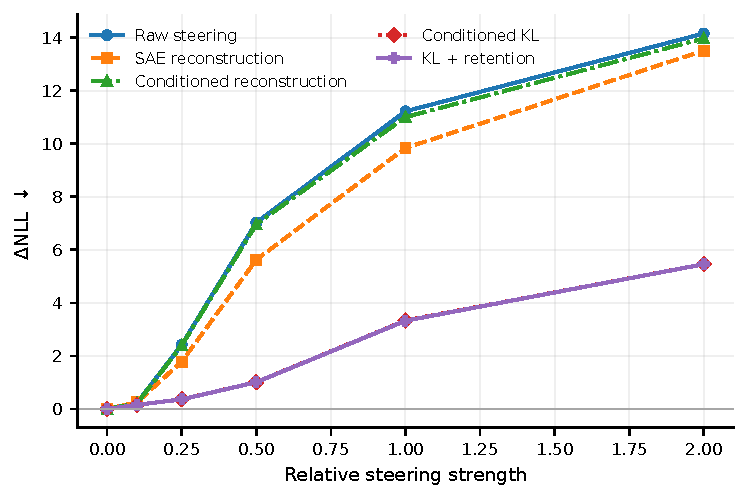
\includegraphics[width=\linewidth]{strength_delta_nll.pdf}
    \caption{Downstream degradation.}
  \end{subfigure}\hfill
  \begin{subfigure}[t]{0.49\textwidth}
    \centering
    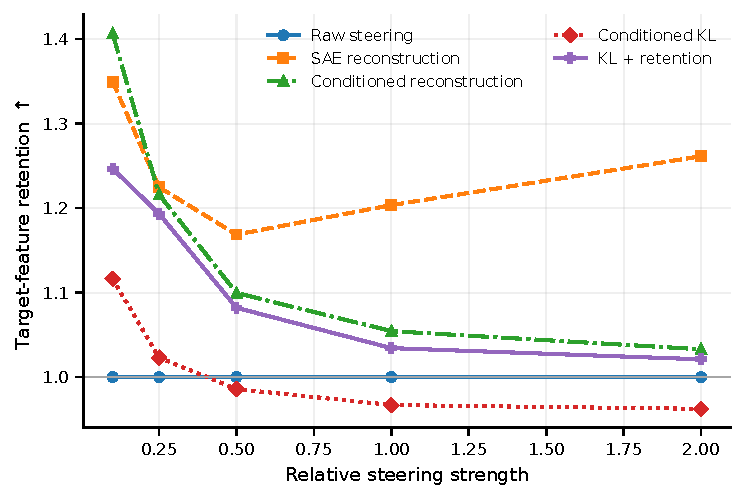
\includegraphics[width=\linewidth]{strength_retention.pdf}
    \caption{Target-feature retention.}
  \end{subfigure}
  \caption{Strength-dependent causal results. Downstream KL objectives provide the main reduction in degradation, while the retention term primarily changes preservation of the target feature. Error summaries and matched comparisons are reported in the accompanying tables.}
  \label{fig:main_curves}
\end{figure*}

\subsection{Unseen-direction holdout}
The designated holdout contains 20 directions and 3,200 matched examples. Relative to raw steering, \method{Conditioned KL + retention} recovers $4.322$ mean $\dNLL$ (95\% CI $[2.927,5.795]$), with all 20 directions improved. KL recovery is $4.331$ (95\% CI $[2.909,5.870]$), again with 20/20 improved. Mechanistic retention increases by $0.108$ (95\% CI $[0.077,0.139]$).

These paired results separate within-family generalization from model selection: direction is the top-level resampling unit, prompts are nested within directions, and the holdout directions are not used to choose the final objective. The result supports generalization across unseen directions from the same SAE family. It does not establish transfer across steering families or models.

The most informative objective comparison is \method{Conditioned KL} versus \method{Conditioned reconstruction}. Switching to KL recovers $4.265$ mean $\dNLL$ (95\% CI $[2.883,5.643]$) and $4.272$ KL (95\% CI $[2.888,5.707]$), with all 20 directions improved. However, retention decreases by $-0.152$ (95\% CI $[-0.181,-0.123]$). Functional matching therefore creates pressure to suppress the intervention, motivating a separate retention objective.

Relative to SAE reconstruction, the selected method recovers $3.636$ mean $\dNLL$ (95\% CI $[2.307,5.165]$), with 19/20 directions improved, but has lower mechanistic retention by $\Delta R=-0.099$. Under the experiment's fixed bounds, its paired hypervolume difference is $\Delta HV=-0.0201$. Thus the selected model does not dominate SAE reconstruction under every Pareto summary.

\subsection{Role of retention}
Adding retention changes validation $\dNLL$ only from $2.0684$ to $2.0626$, while mean retention rises from $1.0109$ to $1.1155$. On holdout, \method{Conditioned KL + retention} versus \method{Conditioned KL} yields $0.0047$ $\dNLL$ recovery (95\% CI $[-0.0049,0.0153]$), providing no evidence for material additional NLL benefit. Retention instead increases by $0.1096$ (95\% CI $[0.0933,0.1298]$), with all 20 directions improved. Downstream KL repairs functionality; retention constrains what repair is allowed to erase.

\subsection{Cross-concept sentiment confirmation}
One independently constructed sentiment direction provides 40 matched examples. The purpose is confirmation, not broad cross-concept generalization. \method{Conditioned reconstruction} is worse than SAE reconstruction by $-1.188$ $\dNLL$ recovery (95\% CI $[-1.329,-1.053]$). Switching from conditioned reconstruction to conditioned KL produces $+1.300$ recovery (95\% CI $[0.972,1.575]$), improves KL by $1.318$, and increases retention by $0.0887$. Relative to raw sentiment steering, \method{Conditioned KL + retention} recovers $1.401$ mean $\dNLL$ (95\% CI $[1.082,1.692]$) and improves retention by approximately $0.087$.

This cross-concept result confirms the KL-over-reconstruction decomposition on one qualitatively different direction. It is reported separately from within-SAE-family generalization. A single sentiment direction cannot support a universal cross-concept claim, even though its paired confidence intervals are informative for this particular intervention.

\begin{figure*}[t]
  \centering
  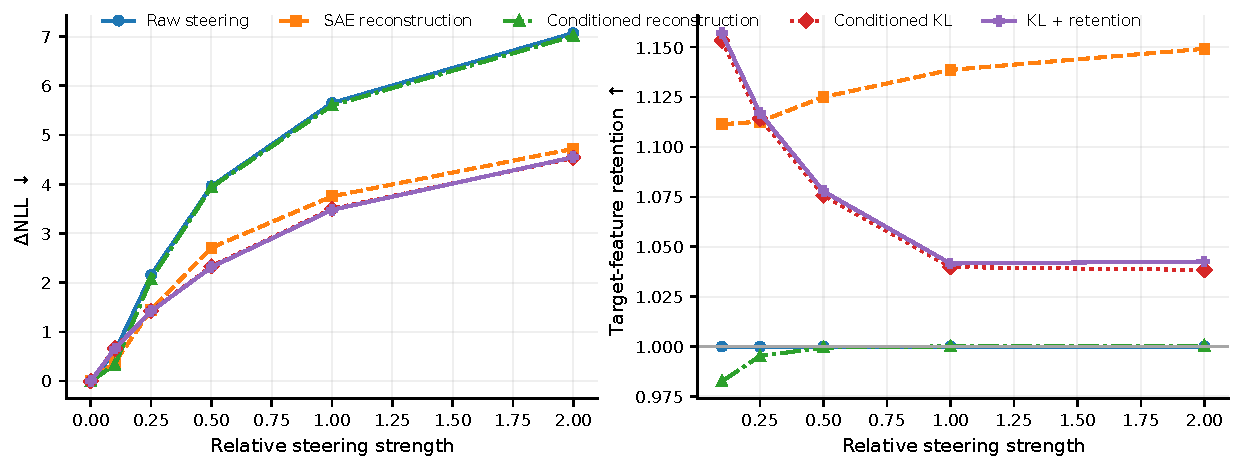
\includegraphics[width=0.90\textwidth]{cross_concept_sentiment_confirmation.pdf}
  \caption{Cross-concept sentiment confirmation. Downstream KL again outperforms conditioned reconstruction, but evidence is limited to one independent direction and 40 matched examples.}
  \label{fig:sentiment}
\end{figure*}

\section{Independent Semantic Evaluation}
The target SAE feature is not equivalent to semantic behavior in generated text. A public SAE feature associated with greeting and welcoming behavior is therefore evaluated by a separate classifier. Its sanity check gives positive mean $0.993$, negative mean $0.00236$, and ROC AUC $1.0$.

Raw semantic score rises from approximately $0.0015$ at zero strength to $0.272$ at strength $1.0$, then falls to $0.089$ at strength $2.0$. The correlation between raw SAE activation and external semantic score is only $\rho=0.17216$; across methods it is $\rho=0.28957$. A negative-control score remains small at weak and moderate strengths but increases at the most aggressive intervention. Keyword masking reduces semantic score by approximately $0.0247$ on average. The external classifier is itself a semantic proxy, not human evaluation.

The non-monotonic response is consistent with an operating regime in which stronger intervention initially increases the classifier-detected property, while aggressive steering introduces degeneration or other classifier-sensitive effects. More importantly, the weak correlations show why intervention-signal preservation and semantic success must be reported as different quantities. Neither the SAE coordinate nor the classifier is promoted to semantic ground truth.

\begin{figure}[t]
  \centering
  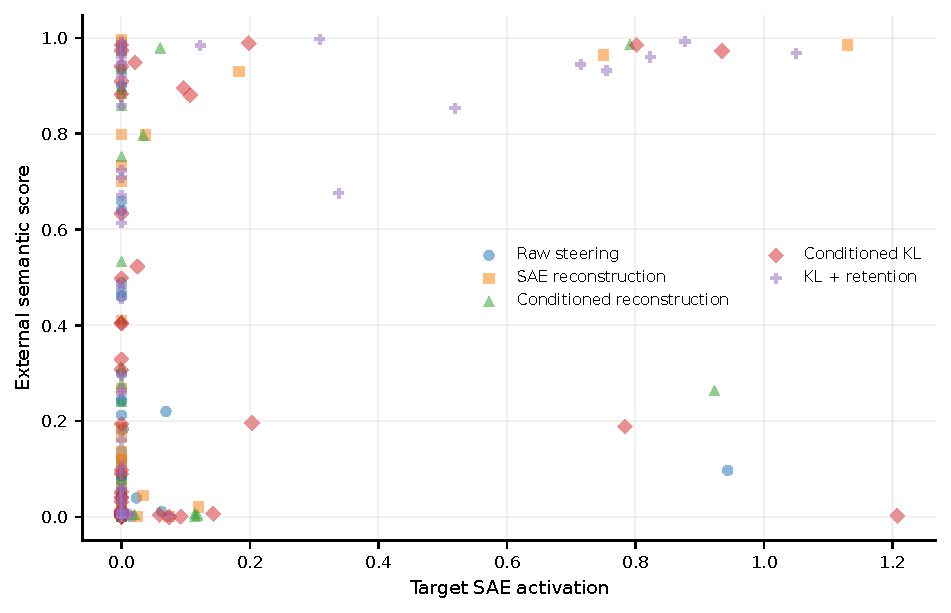
\includegraphics[width=\linewidth]{sae_vs_external_semantic_score.pdf}
  \caption{Weak correspondence between mechanistic SAE activation and the independent output-level semantic proxy. SAE retention should not be interpreted as semantic ground truth.}
  \label{fig:semantic}
\end{figure}

\section{Discussion}
The experiments distinguish state reconstruction from functional reconstruction. The transformer does not consume Euclidean distance; it processes a repaired activation through nonlinear attention, MLP, normalization, and residual computations. This explains why a conditioned reconstruction model can be activation-aware yet functionally weak, while a downstream KL objective yields a large benefit.

Downstream matching alone is incomplete because exact clean-behavior recovery favors removing the steering signal. The resulting task is constrained functional repair: reduce collateral damage without cancelling the intervention. This separation is also visible in free-running generation, where autoregressive compounding prevents the token-level ranking from transferring uniformly, especially at high strengths.

Direction identity matters as well as perturbation magnitude. Across the scored training directions, supplied mean KL damage ranges from approximately $0.786$ to $11.037$, a greater-than-order-of-magnitude spread at common nominal strengths. Layer selection and activation granularity likewise affect steering quality \citep{sun2025layernavigator,feng2026austeer}. This heterogeneity motivates conditioning on $(v,s)$, but the causal ablation shows that metadata alone is not sufficient: the objective must also align repair with downstream function.

Natural-neighbor diagnostics provide a geometric description, not a semantic certificate. Learned activation priors offer a richer route to modeling the residual-stream distribution \citep{luo2026glp}, but proximity to a probable state still does not establish preservation of the intended intervention. A repair that moves an activation toward a high-density clean region can erase the causal signal. The operational requirement is therefore stricter: repair must preserve the intended causal or semantic steering signal, not merely reduce distance to clean activations.

Soft retention and hard projection are both viable within the SAE family. On the unseen holdout, soft relative to hard gives $\dNLL=-0.043$ (95\% CI $[-0.099,0.003]$) and retention $+0.021$ (95\% CI $[-0.012,0.058]$); Pareto uncertainty also crosses zero. On sentiment, hard projection has lower NLL/KL ($\dNLL=-0.072$ and $\Delta\mathrm{KL}=-0.160$ for soft versus hard), while soft retention preserves more signal, $\Delta R=+0.087$ (95\% CI $[0.076,0.097]$). These results establish a tradeoff, not universal superiority.

\section{Limitations}
All primary experiments use GPT-2 Small at one residual-stream layer. The evidence does not establish transfer to larger models, other architectures, or other intervention points. Most directions come from one SAE family: the 20-direction holdout supports within-family generalization, not unrestricted steering generalization. Cross-concept evidence contains one sentiment direction and 40 matched examples.

The main retention metric measures the same SAE feature defining the intervention and is not independent semantic evidence. The external classifier also remains a proxy rather than human evaluation. Free-running generation does not uniformly reproduce the token-level ranking. Finally, fixed-bound Pareto hypervolume depends on the chosen bounds and is explicitly not cross-study comparable.

Generation-level results are secondary because free-running continuation compounds small distributional differences over many autoregressive steps. The present evidence therefore supports immediate downstream distribution repair more strongly than full autoregressive recovery. Human judgments of fluency and semantic success are absent, and neither teacher-forced $\dNLL$ nor classifier score should be substituted for such evaluation.

\section{Conclusion}
Strong steering can induce substantial downstream degradation. Conditioning a reconstruction model on direction and strength does not solve the problem: mean $\dNLL$ remains $6.91$. Direct downstream optimization reduces it to $2.07$. Adding soft retention changes degradation negligibly, from $2.068$ to $2.063$, while increasing mechanistic retention from $1.011$ to $1.115$. The decomposition survives the frozen 20-direction holdout and reappears in one independent sentiment experiment. The supported conclusion is narrow but clear:
\begin{center}
\fbox{\parbox{0.90\columnwidth}{\centering\bfseries Functional steering repair is not activation reconstruction.}}
\end{center}

\bibliographystyle{plainnat}
\setlength{\bibsep}{0pt}
{\footnotesize\bibliography{references}}

\clearpage
\appendix
\section{Calibration and Corruption Geometry}
The standardized corruption construction removes a scale confound by enforcing exact norm and MSE identities. It does not, by itself, show that standardization causes downstream recovery. The recorded analytical and real-batch checks are reported in Section~4.1; duplicate norm and correction-geometry plots are omitted.

\section{Additional Baselines}
Norm-preserving steering tests whether radial growth alone explains degradation. Gaussian denoising tests generic approximately isotropic corruption. SAE reconstruction tests structured corruption without intervention identity. Their aggregate results are already contained in the primary causal-ablation table and strength curves, so duplicate visual summaries are omitted.

\section{Hard Projection}
Hard projection removes the component of the denoiser correction parallel to the steering vector. The main paper reports all supplied uncertainty: neither the SAE holdout nor its Pareto interval supports a universal soft-over-hard claim. Sentiment instead suggests that hard projection can be more aggressive downstream while soft retention preserves more intervention-parallel signal.

\begin{figure*}[t]
  \centering
  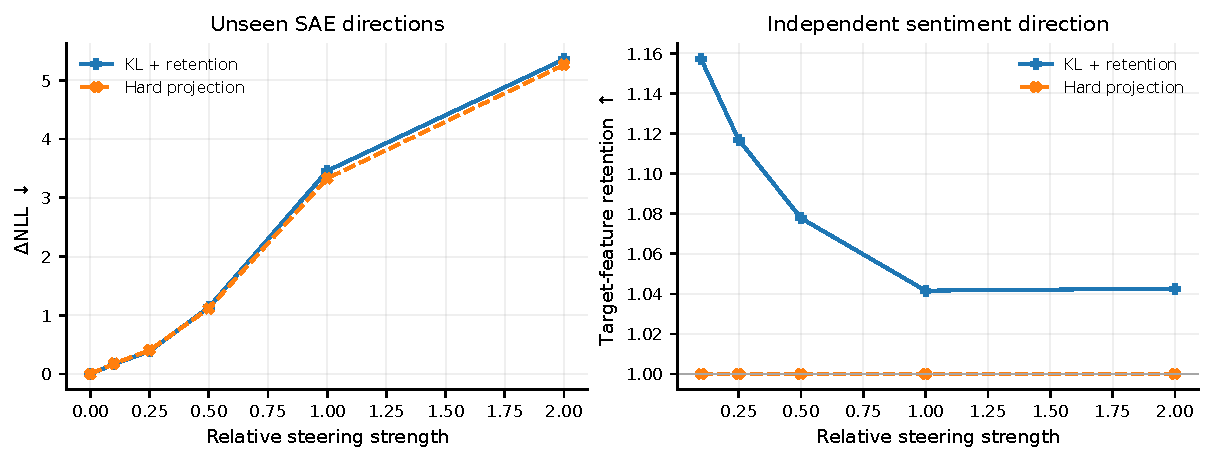
\includegraphics[width=0.88\textwidth]{hard_projection_vs_soft_retention.pdf}
  \caption{Hard projection versus soft learned retention. The SAE holdout does not establish universal dominance; the sentiment direction reveals a downstream-repair versus signal-preservation tradeoff.}
  \label{fig:projection}
\end{figure*}

\section{Harmfulness Heterogeneity}
Training-direction damage varies by more than an order of magnitude: mean KL ranges from approximately $0.786$ to $11.037$. Equal nominal strength therefore does not imply equal downstream disruption, motivating a correction that depends on direction as well as magnitude.

\begin{figure}[t]
\centering
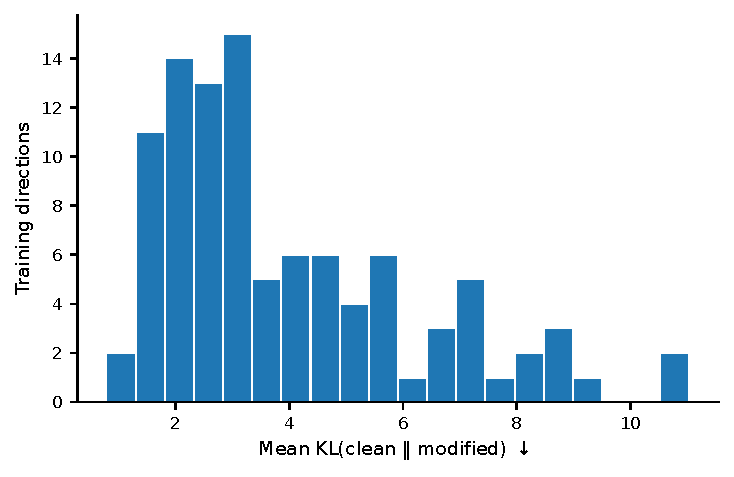
\includegraphics[width=\linewidth]{harmfulness_distribution.pdf}
\caption{Heterogeneity of downstream damage across training SAE directions.}
\label{fig:app_harmfulness}
\end{figure}

\section{Natural-Neighbor Diagnostics}
Nearest-neighbor distance in a PCA projection of clean activations is treated only as a density diagnostic. Moving toward high-density clean regions is not sufficient for semantic correctness; repair must preserve the intended causal signal.

\begin{figure}[t]
\centering
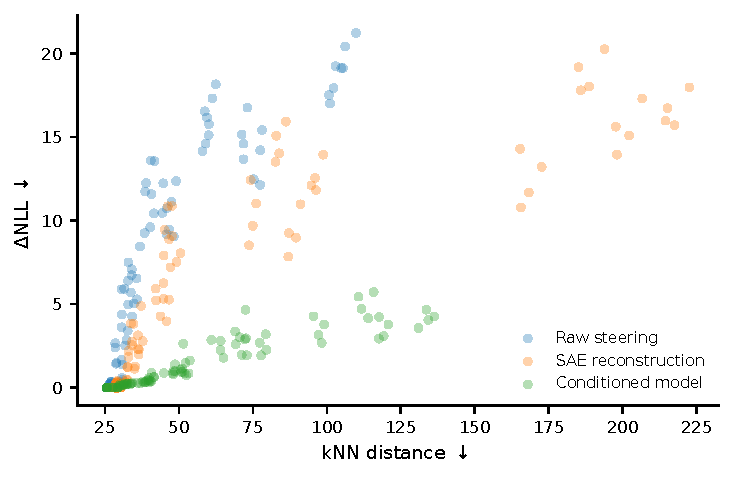
\includegraphics[width=\linewidth]{knn_distance_vs_delta_nll.pdf}
\caption{kNN distance versus $\dNLL$.}
\label{fig:app_neighbors}
\end{figure}

\section{Generation Diagnostics}
Free-running continuations are scored by clean-model continuation NLL, distinct-$n$, repetition, activation norm, and target-feature statistics. These exploratory metrics do not reproduce the teacher-forced ranking uniformly because small distributional differences compound over autoregressive steps.

\section{External Semantic Evaluation Details}
The greeting classifier receives generated text rather than internal model states. The supplied sanity metrics are positive mean $0.993$, negative mean $0.00236$, and ROC AUC $1.0$. Figure~\ref{fig:app_semantic_strength} shows the retained semantic diagnostics.

\begin{figure}[b]
\centering
\begin{subfigure}[t]{0.96\linewidth}
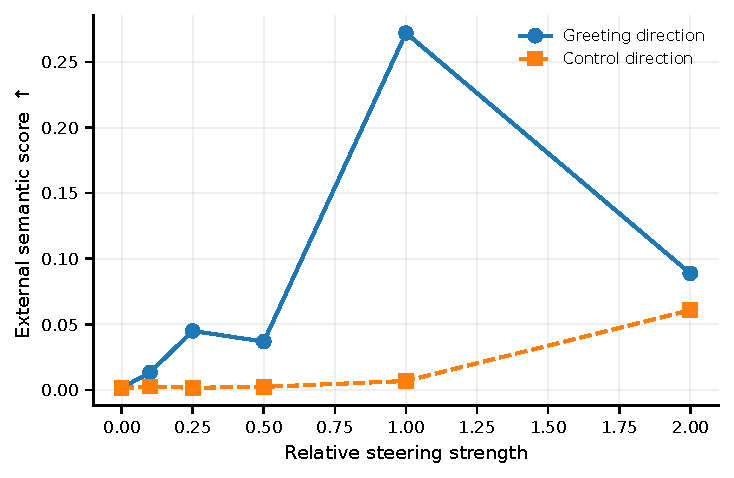
\includegraphics[width=\linewidth]{greeting_vs_control_direction.pdf}
\caption{Greeting feature versus control direction.}
\end{subfigure}\\[3pt]
\begin{subfigure}[t]{0.96\linewidth}
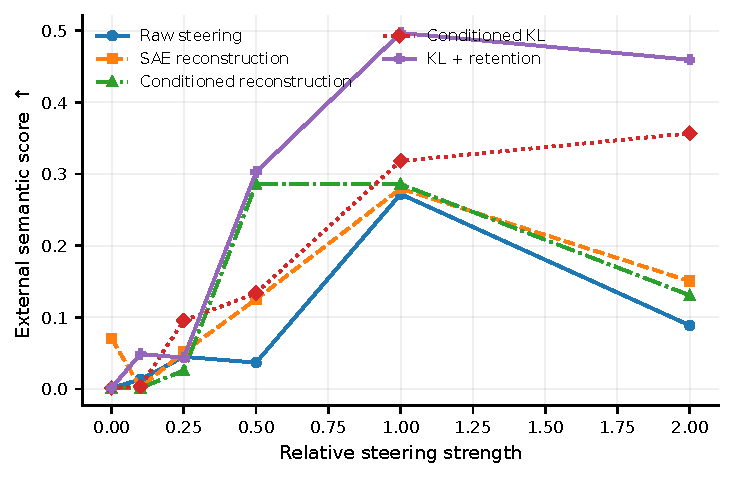
\includegraphics[width=\linewidth]{semantic_score_vs_strength.pdf}
\caption{Semantic score versus strength.}
\end{subfigure}
\caption{External semantic proxy diagnostics.}
\label{fig:app_semantic_strength}
\end{figure}

\section{Additional Tables}
\begin{table}[h]
\centering
\caption{Validation selection among conditioned candidates.}
\small
\begin{tabular}{lrrr}
\toprule
Method & $\dNLL\downarrow$ & KL$\downarrow$ & Ret.$\uparrow$\\
\midrule
Conditioned full & 2.093 & 2.150 & 1.152\\
Conditioned KL & 2.068 & 2.125 & 1.011\\
Conditioned KL + retention & \textbf{2.063} & \textbf{2.120} & 1.115\\
Conditioned reconstruction & 6.906 & 6.942 & 1.162\\
\bottomrule
\end{tabular}
\end{table}

\begin{table}[h]
\centering
\caption{Selected holdout paired effects. Positive recovery means lower degradation for the named method.}
\small
\resizebox{\columnwidth}{!}{%
\begin{tabular}{lrr}
\toprule
Comparison / metric & Effect & 95\% CI\\
\midrule
KL+ret. vs raw, $\dNLL$ & 4.322 & $[2.927,5.795]$\\
KL+ret. vs raw, KL & 4.331 & $[2.909,5.870]$\\
KL+ret. vs raw, retention & 0.108 & $[0.077,0.139]$\\
KL vs reconstruction, $\dNLL$ & 4.265 & $[2.883,5.643]$\\
KL vs reconstruction, retention & -0.152 & $[-0.181,-0.123]$\\
KL+ret. vs KL, $\dNLL$ & 0.0047 & $[-0.0049,0.0153]$\\
KL+ret. vs KL, retention & 0.1096 & $[0.0933,0.1298]$\\
\bottomrule
\end{tabular}
}
\end{table}

\end{document}
